\subsection{Array Non-Uniformity}

\paragraph{Description:}
In our estimates of array performance and sensitivity, we often assume that for an array with number of detectors $N_{\mbox{\scriptsize det}}$, each detector will have common signal-to-noise levels dominated by photon noise, and the sensitivity of the entire array scales as $\sim 1 / \sqrt{N_{\mbox{\scriptsize det}}}$. The measure of signal-to-noise for our detectors is noise-equivalent power, or $NEP$. For transition-edge sensor bolometers, this quantity is a function of parameters like the bias voltage used for each bolometer, the open loop gain $L$, and the thermal parameters $G$ and $T_{\mbox{\scriptsize c}}$, the thermal conductance and critical temperature, respectively, of each detector.

Beyond the TES bolometer itself, within-array variations of important optical parameters like thickness of dielectric layers, relevant to determining signal loss in microwave circuits and thus the optical efficiency of given pixels, have been observed. If we express this number as a temperature-to-power gain $\eta = dT/dP$, then variations in this number will lead to variations in the per-detector $NET$, or noise-equivalent temperature, of the detector. Since $NET \sim \eta NEP$, fluctuations in $\eta$ across the array are relevant for determining how sensitive the overall array is.

In general, achieving uniform sensitivity through fabrication engineering (especially relevant to $G$, $T_{\mbox{\scriptsize c}}$, and $\eta$) has a practical limit. For the former parameters, Advanced ACTPol arrays have shown a very tight distribution, which encourages us to focus on achieving uniform bias parameters over many parameters. \textbf{Add some info/plots on fab uniformity from Shannon's post (link in SPIE progress spreadsheet).} We only have control over the bias currents within ``bias lines'', which provide an identical current to hundreds of TES channels. Figure \ref{expect_biasability} shows the effect of moving from the 12 bias lines per frequency in Advanced ACTPol dichroic arrays to the 4 per frequency being designed in SO.

\begin{figure}[h!]
\centering
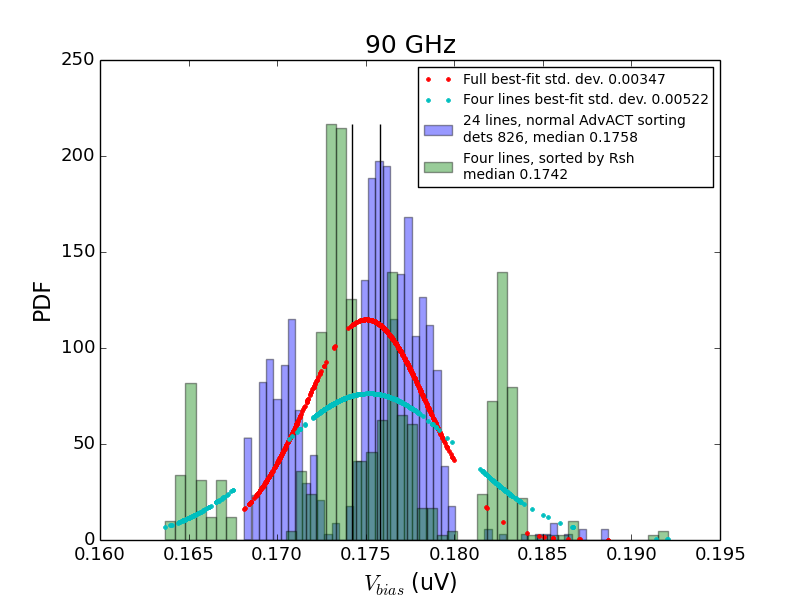
\includegraphics[width=0.4\textwidth]{figures/bias_volt_90GHz_ACTvsSO.png}\quad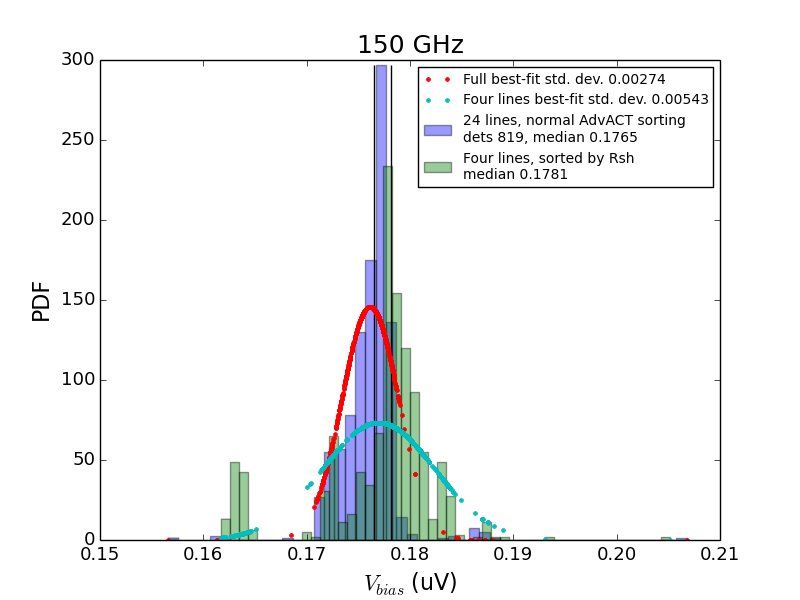
\includegraphics[width=0.4\textwidth]{figures/bias_volt_150GHz_ACTvsSO.png}
\caption{A bias uniformity proxy, detector bias voltage, for 90 and 150 GHz detectors in and AdvACT MF array. The two cases are with 12 bias lines and 4 bias lines per frequency, the latter being the planned for SO.}
\label{expect_biasability}
\end{figure}

However, all of these effects generally do not lead to systematic errors if calibrations are properly performed to bring each channel into agreement on the size of sky signals in CMB temperature units. We may worry more specifically about issues like nonuniform bandpass, but any science will come from array-wide averages of such effects. However, these variations can provide real limits on array performance if they fail to meet certain requirements. They can also set requirements on how well we need to calibrate certain dtector quantities as in the case of nonuniform bandpasses.

\paragraph{Plan to model and/or measure:}
SRF = 2. We have data specifiying the achieved distribution of thermal parameters measured widely across the array, as well as more limited results on efficiency, or $\eta$, and bandpasses. Tuning bias parameters uses as a proxy how well we achieve the target fraction of a detector's normal resistance $R_{\mbox{\scriptsize n}}$. Studying these statistics across a season is another way to learn how uniformly we are able to bias these detectors. Overall, these ``array health monitors'' do not cause systematics on their own, but require calibration issues to leak signal in. If all parameters are known for all channels, non-uniformity is not itself an issue. \textbf{How practical is it to say we should know it for all channels? Some come from IV curves, but others need specific calibration (like the bandpass), in which case measuring the full array may not be possible/practical. Make some comment here on practicality for different cases.} 

\paragraph{Uncertainty/Range:}
Current distributions of thermal parameters are tight, at a level of $\sim$ few \% [Ho SPIE 2016, Choi LTD 2017] \textbf{add these to the .bib file}. Strong trends with radius do not appear intrinsically. Projecting all of these numbers to array sensitivies [Choi LTD 2017] and comparing to the naive estimate based on $N_{\mbox{\scriptsize det}}$ averaging effects may be useful to determine the sensitivity hit.

\paragraph{Parameterization:}
We intend to calculate the sensitivity hit due to realistic nonuniformity around target parameters determined by the Detector TWG.
